\section{Report: F-Secure}

\begin{frame}{New Report from F-Secure}
\begin{minipage}{0.48\textwidth}
\begin{itemize}
	\item Foscam 
	\item 18 vulnerabilities
	\begin{itemize}
		\item Default credentials
		\item Hardcoded credentials
		\item Hidden services
		\item etc.
	\end{itemize}
	\item White label
	\begin{itemize}
		\item At least 14 brands
	\end{itemize}
\end{itemize}

\end{minipage}
%
\hfill
%
\begin{minipage}{0.48\textwidth}
\begin{figure}
	
	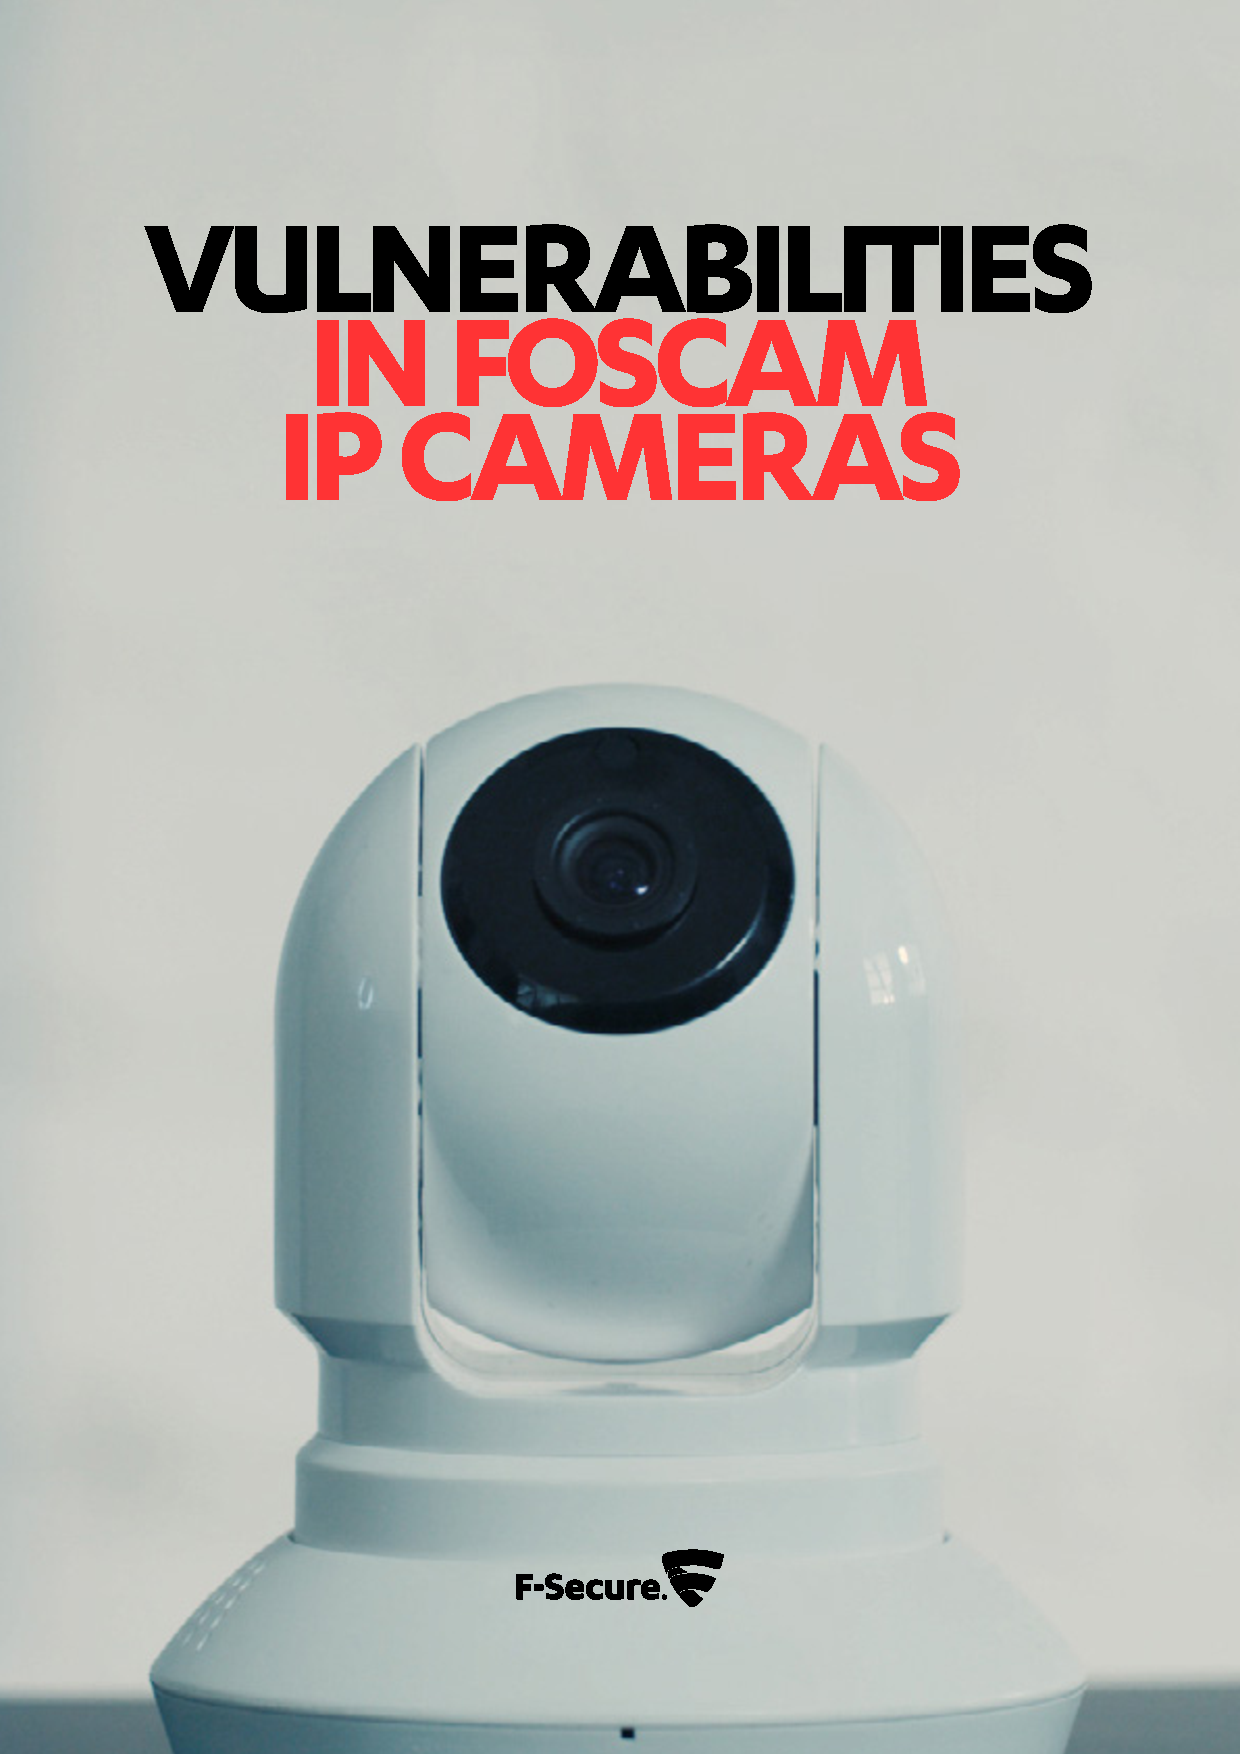
\includegraphics[width=\textwidth]{figs/f-secure}
\end{figure}
\end{minipage}

\end{frame}

\subsection{Recommendations}
\begin{frame}{F-secure Recommendations}

\begin{itemize}
	\item Users
\begin{itemize}
	\item IoT devices on seperate network / VLAN
	\item Always change credentials
\end{itemize}
	\item Corporate
\begin{itemize}
	\item Never assume anything to be secure without evidence
	\item Do security testing before deployment
\end{itemize}
	\item Vendors
\begin{itemize}
	\item Make existing fixes available for all models in a coordinated way
	\item Never trust user input
	\item Remove unused services
	\item Avoid hardcoded credentials
\end{itemize}
\end{itemize}
	
\end{frame}
